\documentclass[11pt,a4paper]{article}
\usepackage[margin=22mm]{geometry}
\usepackage[T1]{fontenc}
\usepackage{lmodern,tabularx,longtable,booktabs,hyperref,xcolor,graphicx,microtype,enumitem,listings}
\usepackage{url}
\usepackage{fancyhdr}
\setlength{\parindent}{0pt}\setlength{\parskip}{6pt}
\setlist{itemsep=2pt,topsep=3pt}
\emergencystretch=3em
\hypersetup{colorlinks=true,linkcolor=black,urlcolor=blue!60!black}
\newcolumntype{L}{>{\raggedright\arraybackslash}X}
\newcommand{\entry}[2]{\textbf{#1:} #2\par}
\newcommand{\code}[1]{\texttt{\detokenize{#1}}}
\pagestyle{fancy}\fancyhf{}\fancyhead[L]{\small 23CSE455 | Banking case study}\fancyhead[R]{\small Source-backed analysis}\fancyfoot[C]{\thepage}
\setlength{\headheight}{14pt}
\lstset{basicstyle=\ttfamily\footnotesize,breaklines=true,frame=single,columns=fullflexible}
\begin{document}
\begin{center}
{\Large\textbf{23CSE455 Design Patterns}}\\[6pt]
{\LARGE\textbf{Case Study Report}}\\[8pt]
{\large Design Pattern Usage and Evolution\\in an ASP.NET Core Banking Application}
\end{center}
\entry{Team}{Banking team code not supplied; confirm before submission.}
\entry{Application}{BankSystem, a real open-source ASP.NET Core banking application. Faculty approval has not been supplied.}
\entry{Date}{2026-10-24}
\entry{Submission repository}{\url{https://github.com/aswathymohan-amrita/23CSE455_DP_CaseStudy}}
\entry{Package}{\code{BankingCaseStudy/}; prepared for the user to upload. No GitHub push was performed.}
\textbf{Students and contributions}\par
The exact banking-team roster, roll numbers, batch and individual contributions were not provided. They are deliberately not copied from the unrelated healthcare team or invented. Add the verified details in \code{team.json} and this cover before submission.

\textbf{Study summary}\par
This study inspects the pinned BankSystem source, maps three baseline pattern types to six named collaborations, implements three changes inside the application, and compares five verified pattern types through twenty implementations in Java, Python, JavaScript and C++. The changes add a recovery-code second factor, bill payments with atomic local posting, and a configurable high-value rule.

\textbf{Verification summary}\par
The original service suite passed 129/129 on the baseline and 129/129 against the changed production assemblies. The feature suite passed 26/26; its tests include SQLite rollback and actual Identity recovery-code consumption. Twenty portable implementations passed 92/92 shared cases. These results do not claim a live SQL Server/browser/provider deployment.

\textbf{Evidence boundary}\par
The original source is separated from student-added changes; intermediate versions and exact patches are retained. Team/faculty sign-off, a complete raw AI conversation export with access-tier evidence, and a GitHub screenshot remain owner-supplied submission items. No human verification or historical LLM experiment is fabricated.
\clearpage
\section{Application and architecture}
\entry{Original source}{\url{https://github.com/banksystembg/BankSystem}. Exact baseline: \code{9af0ff8e42e4769d370203ae681e913339ec0121}. Access date: 2026-10-24. License: MIT, retained with both source versions.}
\entry{Environment}{ASP.NET Core/.NET Core 3.1, C\# 8, .NET Standard 2.1 class libraries; EF Core SQL Server and Identity 3.1.12; AutoMapper 10.1.1; SendGrid 9.10.0.}
\entry{Scope}{Four bank service collaborations and listed controller clients, account/login/2FA pages, transfer and payment boundaries, notification adapter, security-header builder, models and context. Dependency internals, DemoShop and CentralApi internals are outside the pattern count.}
\entry{Source integrity}{Included baseline files are byte-identical to the pinned upstream. Seven configuration/workflow files are omitted, including upstream example RSA private-key material. The exact omissions and hashes are recorded under \code{data/}. No dependencies, generated binaries or private local configuration are delivered.}
\begin{center}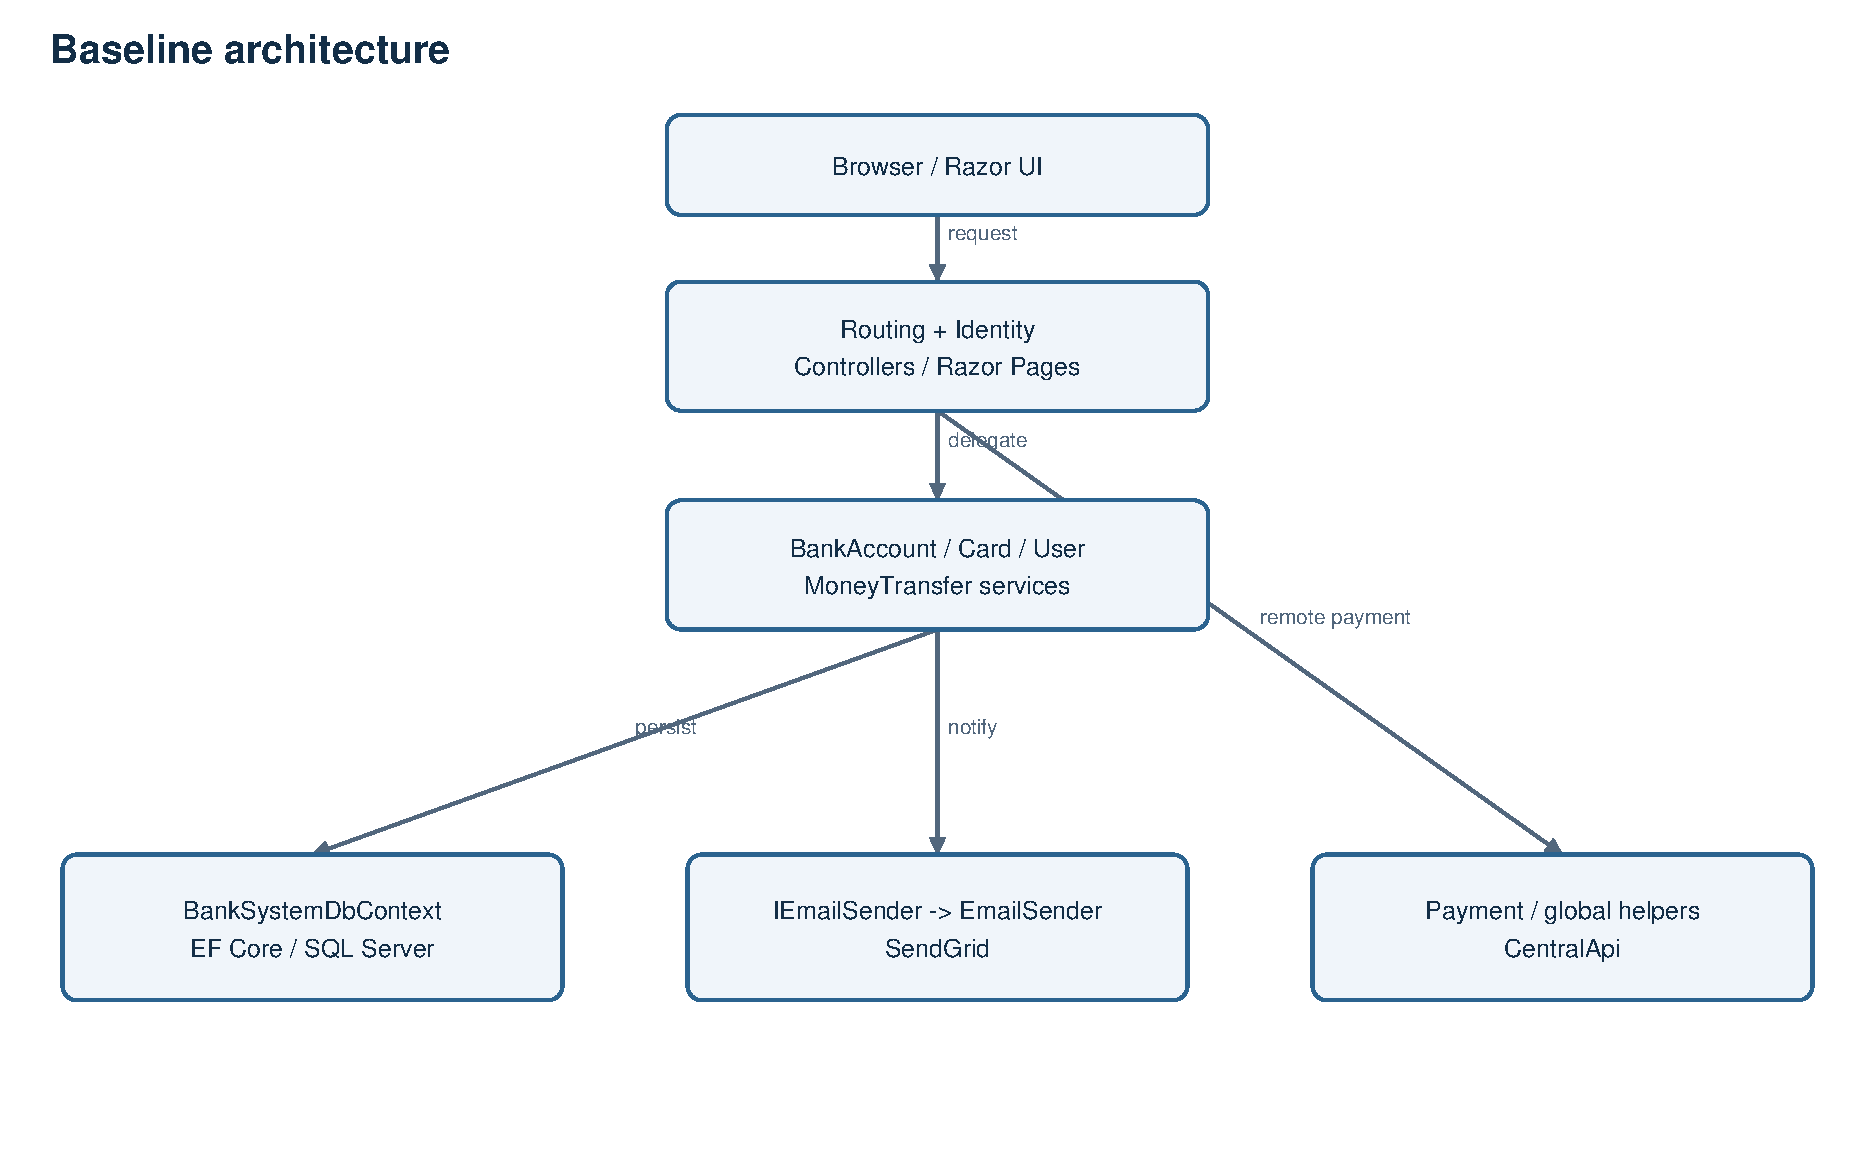
\includegraphics[width=.95\linewidth]{Part1/pattern_architecture/baseline.pdf}\par{\small Figure 1. Original request path and persistence/notification boundaries.}\end{center}
\entry{Request flow}{A browser request reaches routing, Identity and a controller or Razor Page. The controller calls a service interface. Its implementation queries or updates EF entities. MoneyTransferService saves an account balance and one signed transfer record, then directly calls the email adapter. Global/direct/card paths also use CentralApi helpers.}
\entry{Run instructions}{The root README contains dependency/setup, build, test, configuration and web-run commands. Compilation succeeded. Native service tests executed on .NET runtime 3.1.32. The web application was not launched against SQL Server and external providers end-to-end.}
\clearpage
\subsection{Investigation of all assigned areas}
\begin{tabularx}{\linewidth}{@{}p{29mm}L@{}}\toprule
Area & Source-backed finding\\\midrule
Account management & BankAccountsController delegates to IBankAccountService; BankAccountService validates, generates account identifiers and persists EF models.\\
Authentication & LoginModel uses Identity password sign-in; LoginWith2faModel already supports an authenticator. CH01 adds recovery codes rather than claiming 2FA itself is new.\\
Transactions & MoneyTransferService stores a signed ledger row and changes balance. Positive and negative values represent incoming and outgoing postings.\\
Fund transfer & InternalController calls the original posting service twice. These are separate saves; CH02 replaces the internal flow with a transaction-bound service.\\
Payment & PaymentsController and Api/CardPaymentsController implement direct/card boundaries with CentralApi. CH02 adds configured local utility billers.\\
Fraud detection & Ownership, balance, Identity lockout and request-signature checks exist. A configurable linked risk-rule chain was not identified in the selected baseline; CH03 introduces one.\\
Notification & EmailSender converts the application contract to SendGrid message calls and status results. Calling it directly is not Observer.\\
\bottomrule\end{tabularx}
\entry{Evidence index}{\path{Part1/evidence/module_map.md} supplies exact module paths; \path{data/patterns.csv} maps every counted participant to source locations.}
\textbf{Baseline limitation affecting the changes}\par
The original internal controller first posts the debit and then the credit through two service calls. A failure between them can leave inconsistent balances. Extracting the atomic service changes failure behavior intentionally while preserving ordinary successful internal transfers. The original global and direct-payment flows remain separate; this study does not claim they were repaired by the local refactoring.
\textbf{Legacy technology scope}\par
The project targets an older runtime and package set. A successful compile is not a security certification. The captured build reports an end-of-support framework warning and an AutoMapper package advisory. Modernizing the whole framework would be a separate change with its own regression and migration scope.
\clearpage
\section{Part 1: Pattern discovery}
\entry{Method}{Trace contracts, concrete participants, calls and data flow in the selected source. Class names alone are insufficient. Record origin and category; reject unsupported GoF labels. Keep application patterns distinct from dependency internals.}
\subsection{Totals at the baseline}
\begin{tabularx}{\linewidth}{@{}p{75mm}L@{}}\toprule
Measure & Result\\\midrule
Confirmed pattern types & 3: Adapter, Builder, Service Layer\\
Named collaborations & 6: one Adapter, one Builder, four service collaborations\\
Concrete variable-role classes & 6\\
Unique mapped local source symbols & 22; dependency symbols excluded\\
Rejected / uncertain observations & 3 rejected and 1 uncertain; separate from confirmed totals\\
\bottomrule\end{tabularx}
\subsection{Pattern inventory}
\begin{tabularx}{\linewidth}{@{}p{24mm}Lp{16mm}p{16mm}@{}}\toprule
Pattern & Instance names & Instances & Concrete\\\midrule
Adapter & Notification transport & 1 & 1\\
Builder & Security header policy & 1 & 1\\
Service Layer & Account administration; Card administration; User profile lookup; Transfer posting & 4 & 4\\
\bottomrule\end{tabularx}
\entry{Counting rule}{Each named independent collaboration is one instance. Methods and concrete alternatives do not create extra instances. Service Layer is architectural, not a GoF pattern. The CSV includes its four deliberately named service collaborations consistently across snapshots.}
\begin{tabularx}{\linewidth}{@{}p{48mm}L@{}}\toprule
Candidate & Decision and reason\\\midrule
Observer & Rejected: direct email invocation; no subscription/publication structure mapped.\\
Custom Repository / Unit of Work & Rejected in application scope: direct DbContext usage; framework internals not counted as custom classes.\\
Singleton & Rejected: static mapping cache is in excluded test setup.\\
Framework middleware Chain/Decorator & Uncertain classification outside counted dependency scope; not confused with the explicit CH03 application risk chain.\\
\bottomrule\end{tabularx}
\clearpage\subsection{Records 1--2: structural and creational collaborations}
\subsubsection*{Notification transport}
Adapter | Structural (GoF) | Origin: upstream application; provider calls use a dependency.

\begin{tabularx}{\linewidth}{@{}p{33mm}L@{}}\toprule
Role & Actual source participant\\\midrule
Target & IEmailSender\\
Adapter & EmailSender\\
Client & MoneyTransferService\\
Client & RegisterModel\\
Client & SendEmailVerificationModel\\
\bottomrule\end{tabularx}
Application IEmailSender accepts receiver/subject/body. EmailSender builds SendGrid message objects, delegates to SendGridClient and converts Accepted/exception to a boolean. SendGridClient and MailHelper are dependency adaptees, not new application classes.

\entry{Verification}{Confirmed by source inspection; transport behavior is reduced and exercised through common Adapter fixtures, and policy construction through Builder fixtures. These portable tests do not call live SendGrid or the original middleware host. Human review remains pending.}
\entry{Evidence}{See the corresponding row in \path{data/patterns.csv} for qualified names and exact file ranges.}
\subsubsection*{Security header policy}
Builder | Creational (GoF) | Origin: upstream application; provider calls use a dependency.

\begin{tabularx}{\linewidth}{@{}p{33mm}L@{}}\toprule
Role & Actual source participant\\\midrule
ConcreteBuilder & SecurityHeadersBuilder\\
Product & SecurityHeadersPolicy\\
Director & Startup\\
Consumer & SecurityHeadersMiddleware\\
\bottomrule\end{tabularx}
Startup assembles security settings through chained builder calls. Builder accumulates additions/removals in a SecurityHeadersPolicy; middleware consumes that product. No abstract Builder interface is declared.

\entry{Verification}{Confirmed by source inspection; transport behavior is reduced and exercised through common Adapter fixtures, and policy construction through Builder fixtures. These portable tests do not call live SendGrid or the original middleware host. Human review remains pending.}
\entry{Evidence}{See the corresponding row in \path{data/patterns.csv} for qualified names and exact file ranges.}
\clearpage
\begin{center}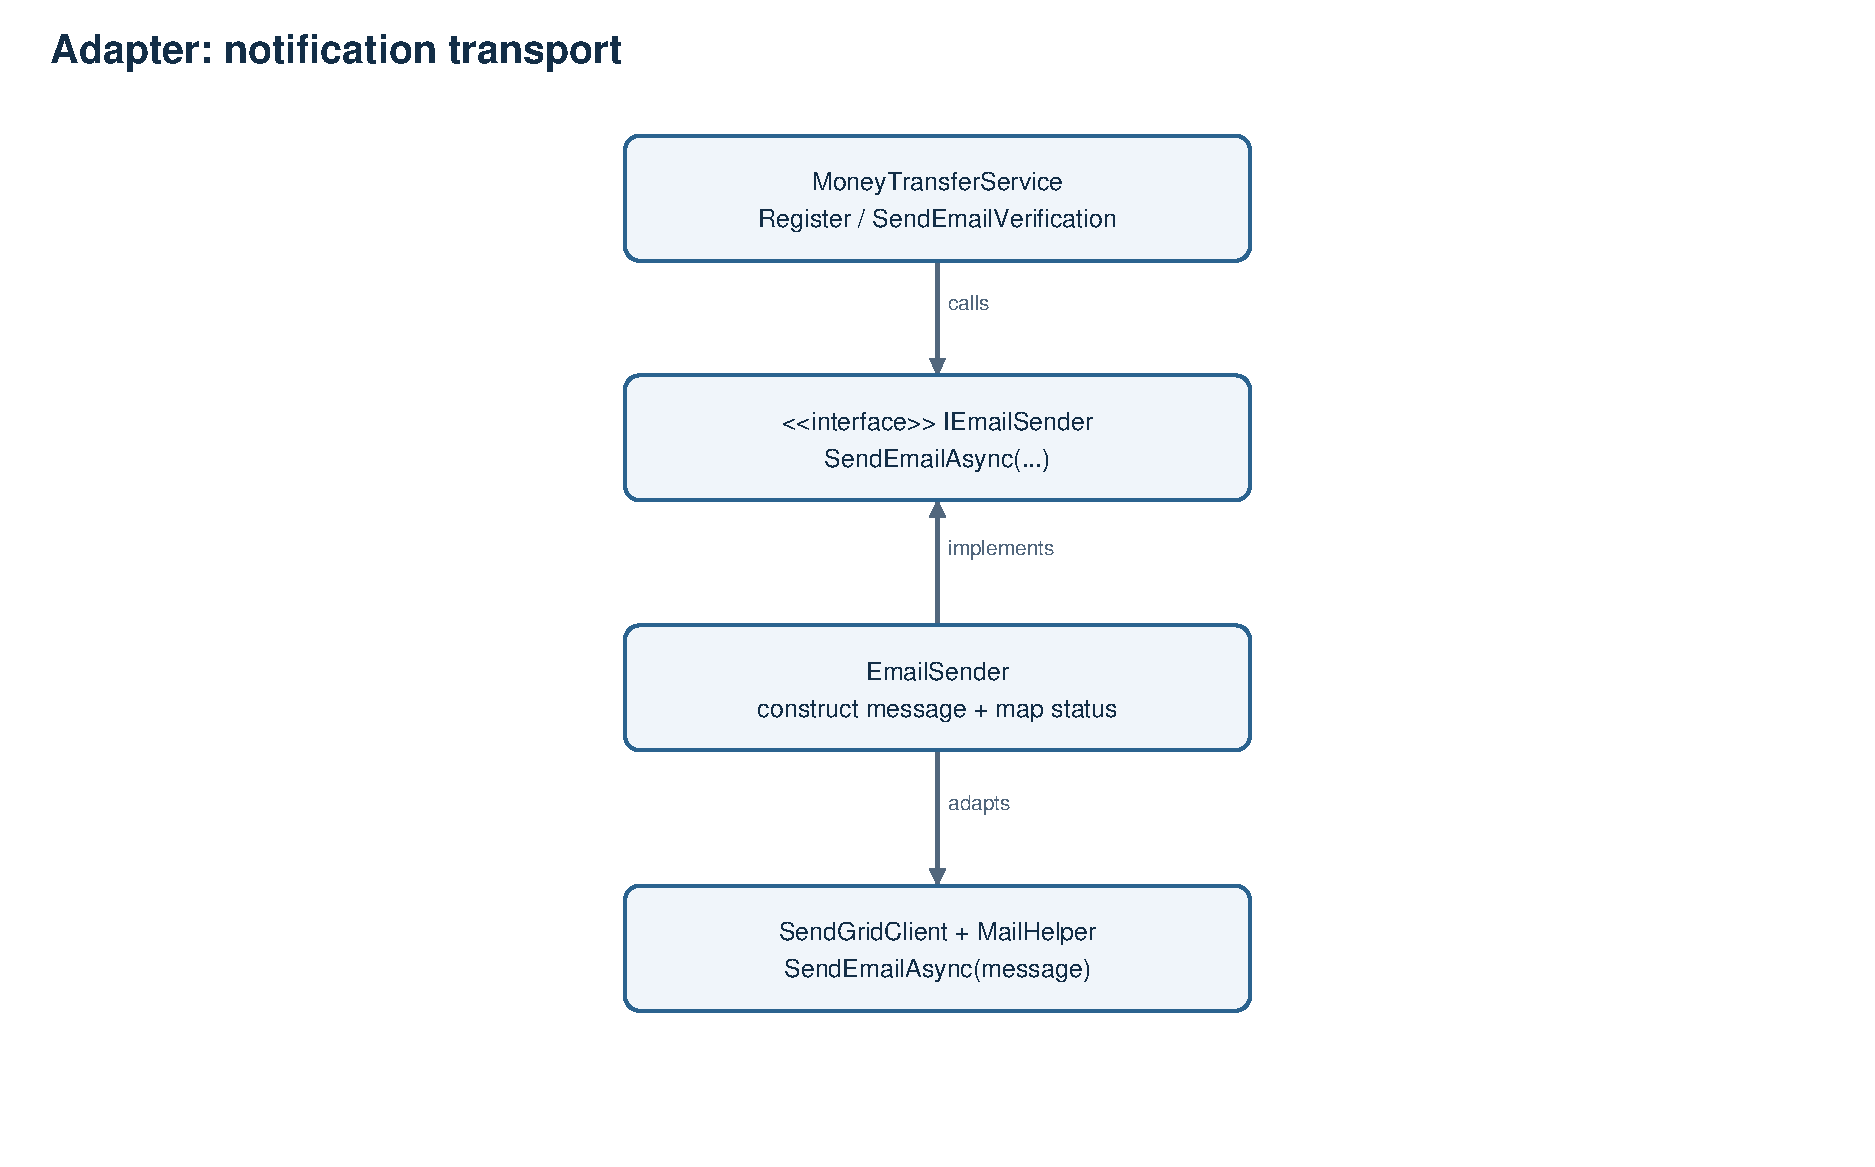
\includegraphics[width=.88\linewidth]{Part1/pattern_architecture/adapter.pdf}\par{\small Figure 2. Notification Adapter roles and provider translation.}\end{center}
\begin{center}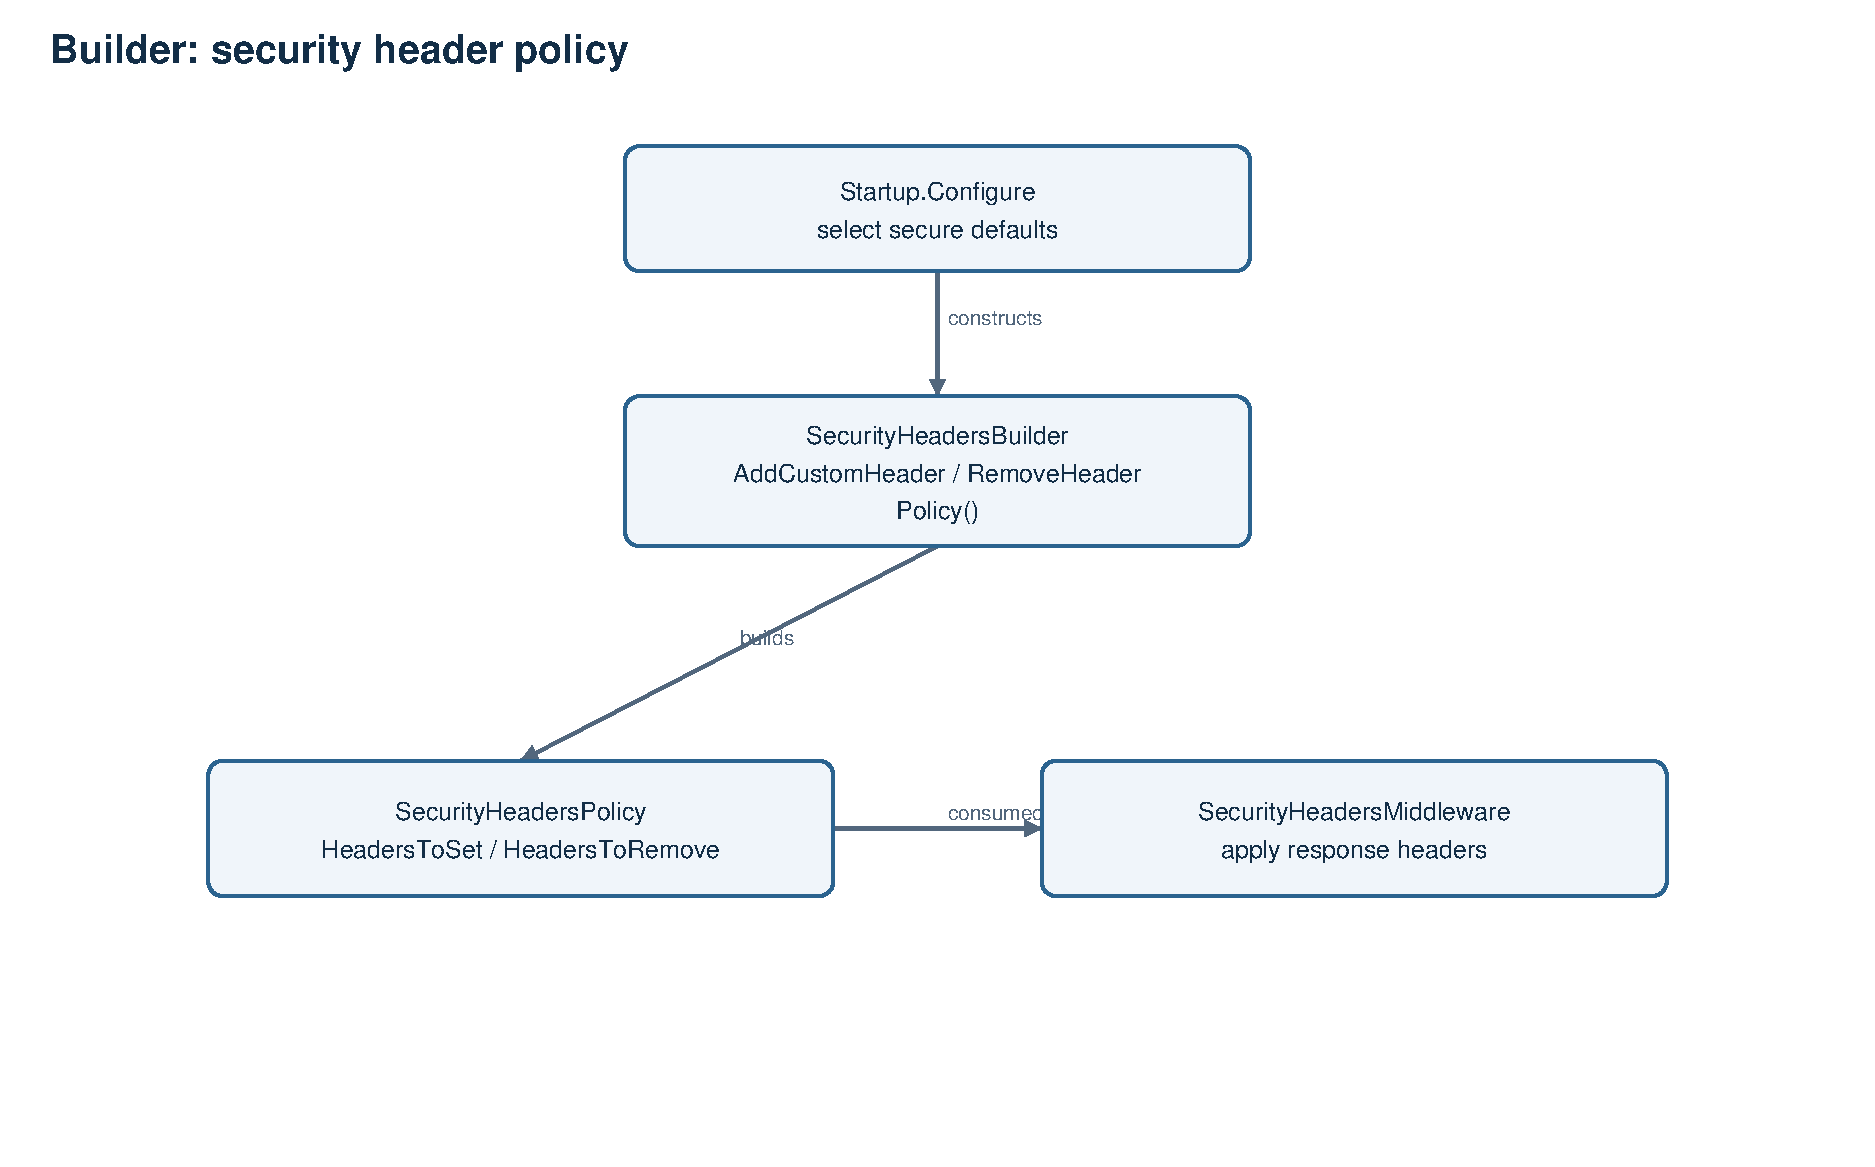
\includegraphics[width=.88\linewidth]{Part1/pattern_architecture/builder.pdf}\par{\small Figure 3. Security-header Builder and its product.}\end{center}
\clearpage\subsection{Records 3--6: application services}
\subsubsection*{Account administration}
\begin{tabularx}{\linewidth}{@{}p{38mm}L@{}}\toprule
Role & Actual participant\\\midrule
Service contract & IBankAccountService\\
Service implementation & BankAccountService\\
Scoped client & BankAccountsController\\
Base & BaseService\\
Persistence & BankSystemDbContext\\
\bottomrule\end{tabularx}
BankAccountsController delegates domain operations to IBankAccountService; BankAccountService coordinates validation or data access through the shared context. Counted as one named service collaboration, not one instance per method. EF Core internals and dependency-injection registration are not additional GoF instances.

\subsubsection*{Card administration}
\begin{tabularx}{\linewidth}{@{}p{38mm}L@{}}\toprule
Role & Actual participant\\\midrule
Service contract & ICardService\\
Service implementation & CardService\\
Scoped client & CardsController\\
Base & BaseService\\
Persistence & BankSystemDbContext\\
\bottomrule\end{tabularx}
CardsController delegates domain operations to ICardService; CardService coordinates validation or data access through the shared context. Counted as one named service collaboration, not one instance per method. EF Core internals and dependency-injection registration are not additional GoF instances.

\subsubsection*{User profile lookup}
\begin{tabularx}{\linewidth}{@{}p{38mm}L@{}}\toprule
Role & Actual participant\\\midrule
Service contract & IUserService\\
Service implementation & UserService\\
Scoped client & GlobalController\\
Base & BaseService\\
Persistence & BankSystemDbContext\\
\bottomrule\end{tabularx}
GlobalController delegates domain operations to IUserService; UserService coordinates validation or data access through the shared context. Counted as one named service collaboration, not one instance per method. EF Core internals and dependency-injection registration are not additional GoF instances.

\subsubsection*{Transfer posting}
\begin{tabularx}{\linewidth}{@{}p{38mm}L@{}}\toprule
Role & Actual participant\\\midrule
Service contract & IMoneyTransferService\\
Service implementation & MoneyTransferService\\
Scoped client & InternalController\\
Base & BaseService\\
Persistence & BankSystemDbContext\\
\bottomrule\end{tabularx}
InternalController delegates domain operations to IMoneyTransferService; MoneyTransferService coordinates validation or data access through the shared context. Counted as one named service collaboration, not one instance per method. EF Core internals and dependency-injection registration are not additional GoF instances.

\entry{Verification}{Confirmed application-service collaborations. The original suite passes 129/129 cases. Exact qualified symbols, source-file ranges and concrete-role audit are in the canonical dataset and \path{Part1/evidence/participant_audit.csv}.}
\clearpage
\begin{center}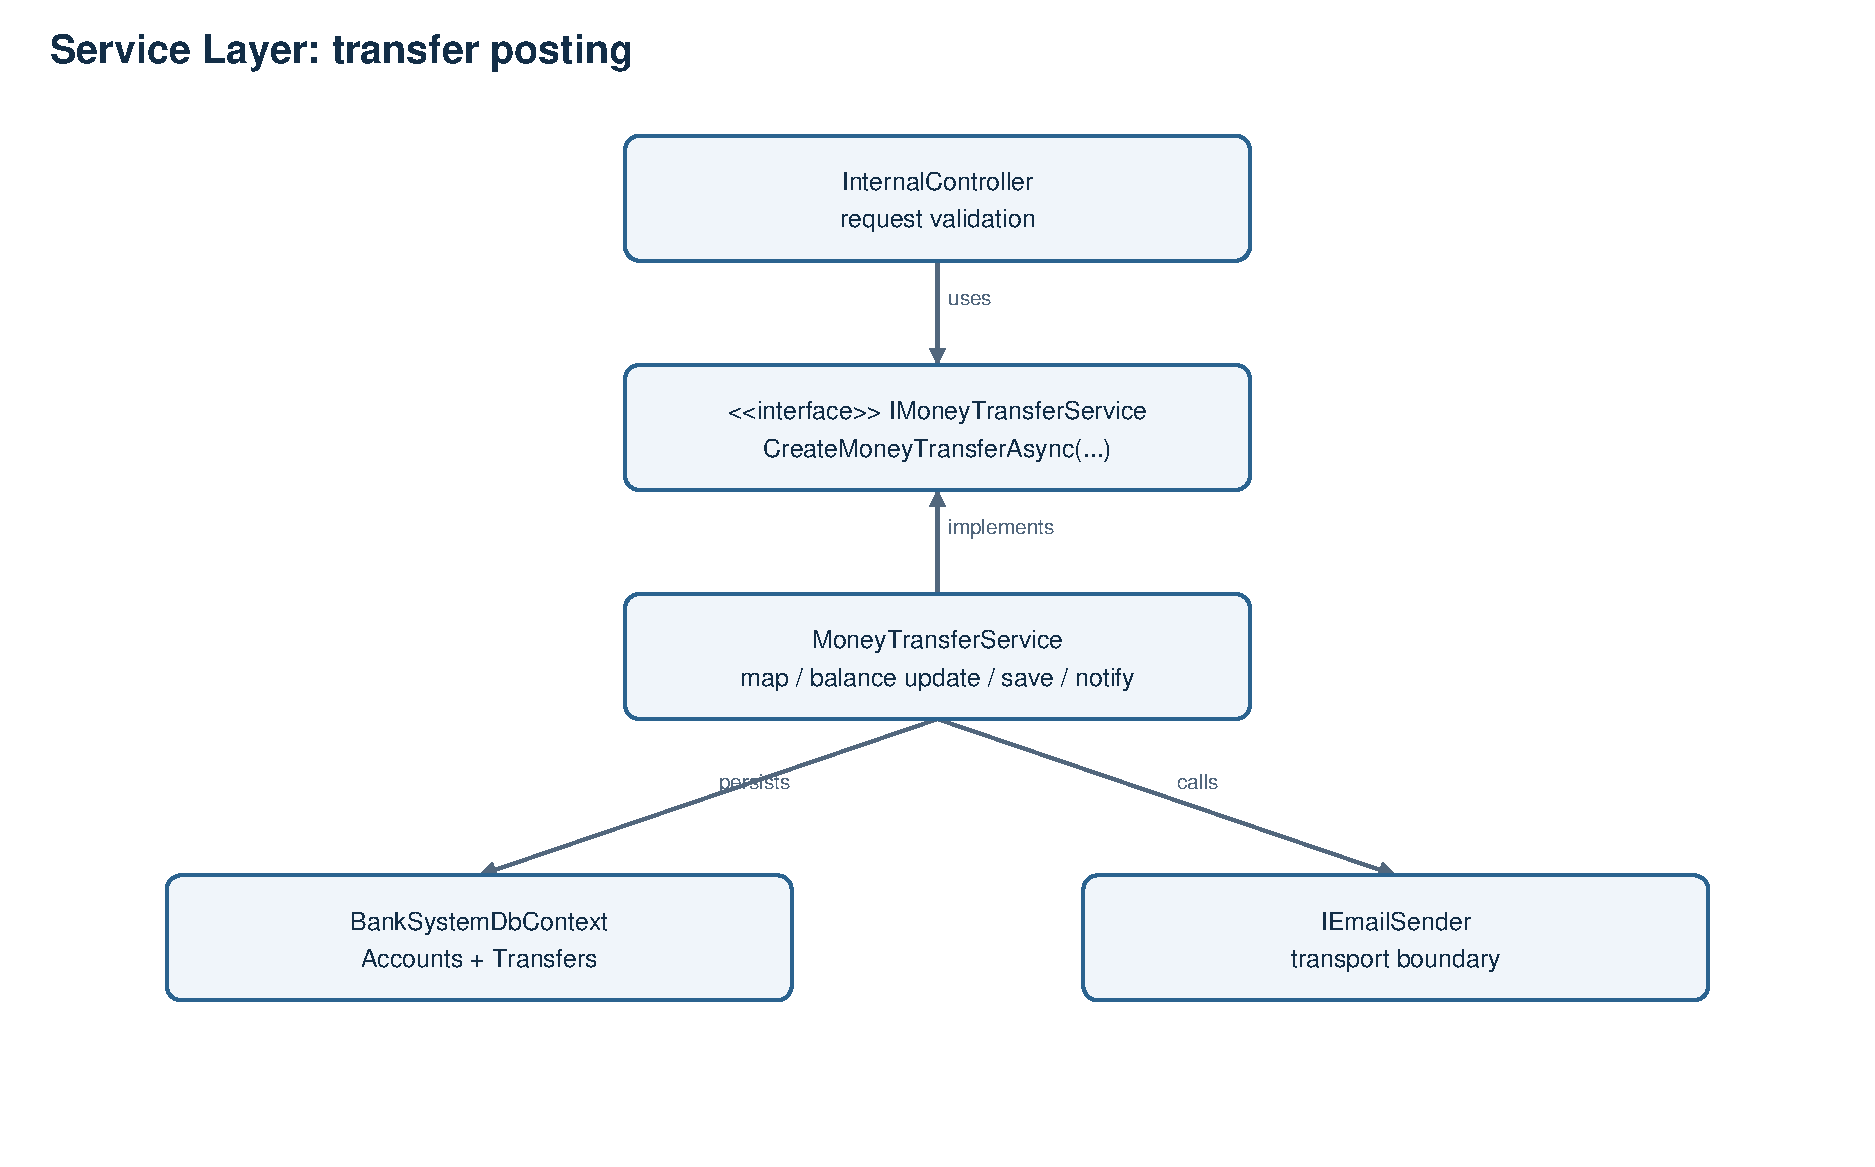
\includegraphics[width=.9\linewidth]{Part1/pattern_architecture/service_layer.pdf}\par{\small Figure 4. The original transfer-posting service boundary.}\end{center}
\textbf{Representative original code evidence}\par
\begin{lstlisting}[language={[Sharp]C}]
userAccount.Balance += dbModel.Amount;
this.Context.Update(userAccount);
await this.Context.Transfers.AddAsync(dbModel);
await this.Context.SaveChangesAsync();
\end{lstlisting}
This exact sequence is in \code{MoneyTransferService.CreateMoneyTransferAsync}. It coordinates a use case, persistence and notification. It does not by itself establish Observer, Repository, Strategy or an atomic two-account transfer. The service can accept signed postings; the controller supplies the account-ownership and sufficient-funds checks for the original internal flow.

\textbf{Source location convention}\par
Each participant entry in \code{patterns.csv} uses a team-relative source path and a line range. A shared file can contain several actual classes; every role names its real qualified symbol. The ranges cover declaration files, not guessed line numbers. Dependency participants such as SendGridClient are explicitly identified as external and excluded from source-symbol counts.
\clearpage
\section{Part 2: Evolution and refactoring}
\subsection{CH01: recovery-code second factor}
\entry{Requirement}{Introduce an alternative to an unavailable authenticator while preserving the existing password and pending-two-factor user flow. A recovery code can be used once; generating a replacement set invalidates the old set.}
\entry{Implementation}{The existing LoginWith2faModel selects AuthenticatorSecondFactor or RecoverySecondFactor behind ISecondFactorStrategy. SecondFactorContext rejects blank input and delegates. RecoveryCodesModel requires authorization, password confirmation, enabled 2FA and lockout checks before generating ten codes.}
\entry{Pattern effect}{New Strategy instance: Second-factor login. Six baseline instances are preserved. Identity performs cryptographic/credential operations; the student code does not invent a token verifier.}
\entry{Refactoring}{Extract Strategy from direct authenticator invocation. The context and page are independent of the selected second-factor algorithm; provider choice remains at the composition boundary.}
\entry{Before/after}{Original snapshot to after\_change1. Exact patch, saved intermediate source and SHA-256 manifest: \path{Part2/changes/Change1/}.}
\begin{center}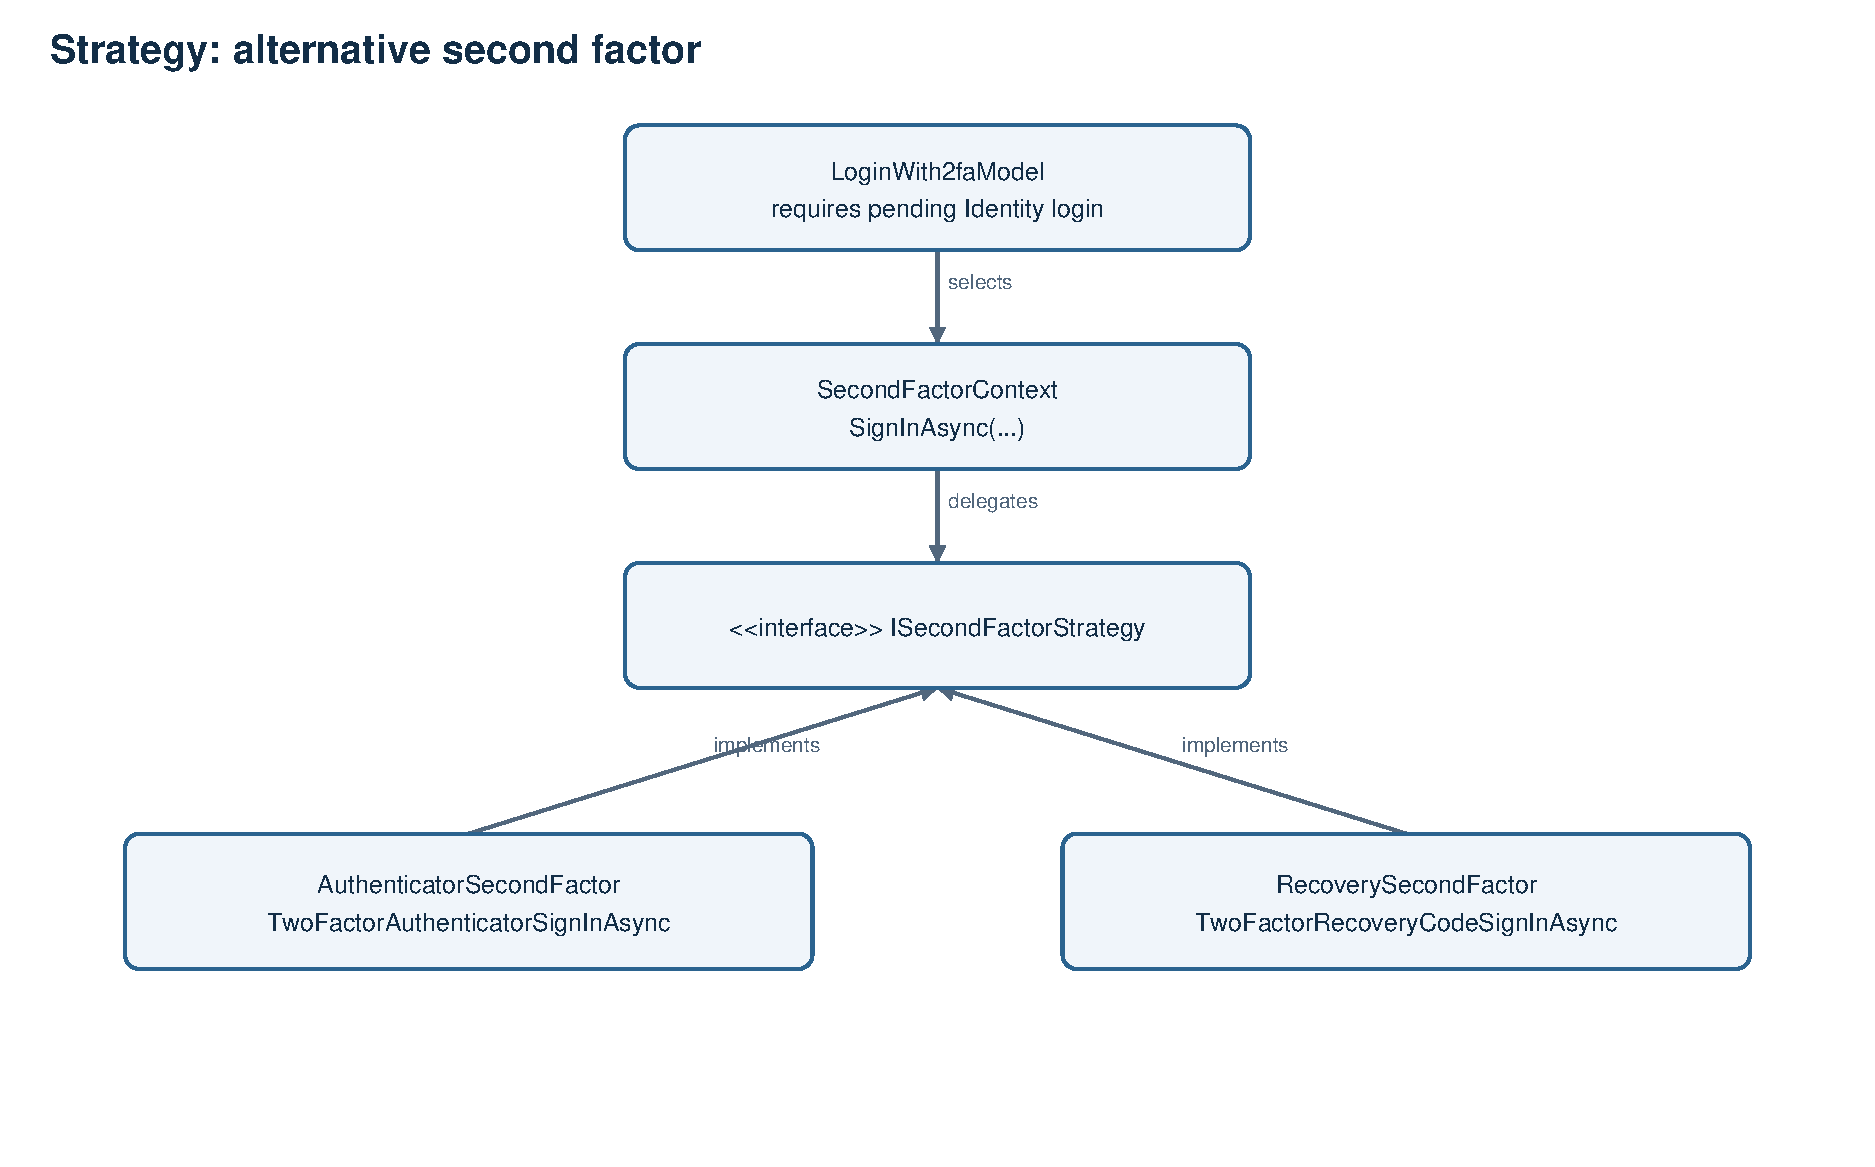
\includegraphics[width=.88\linewidth]{Part2/diagrams/strategy.pdf}\par{\small Figure 5. Two concrete second-factor strategies behind one context.}\end{center}
\entry{Acceptance evidence}{Native tests cover original authenticator-code normalization, recovery-provider delegation, blank/failed code handling and actual UserManager recovery-code single use/replacement. The full browser cookie/antiforgery flow is not claimed tested.}
\clearpage
\subsection{CH02: bill payments and atomic posting}
\entry{Requirement}{Add BillPayment as a persisted transaction type. An authenticated payer chooses an approved configured biller. Source ownership, valid amount, destination and funds must be checked before two balances and paired entries are changed.}
\entry{Implementation}{BillPaymentsController maps electricity/water biller names to configured account identifiers. InternalTransferService performs both entries in one serializable EF transaction. A migration adds TransactionType with Transfer as the default.}
\entry{Real refactoring}{The existing InternalController no longer executes debit and credit through separate calls. It delegates to the same new service as the bill form. Ordinary successful transfers are preserved; partial-failure behavior is intentionally corrected.}
\entry{Pattern effect}{New Service Layer instance: Atomic internal payment. The old Transfer posting collaboration remains for other flows. Notification transport gains the new service as a client.}
\entry{Before/after}{after\_change1 to after\_change2. Patch, intermediate source and hashes: \path{Part2/changes/Change2/}.}
\begin{center}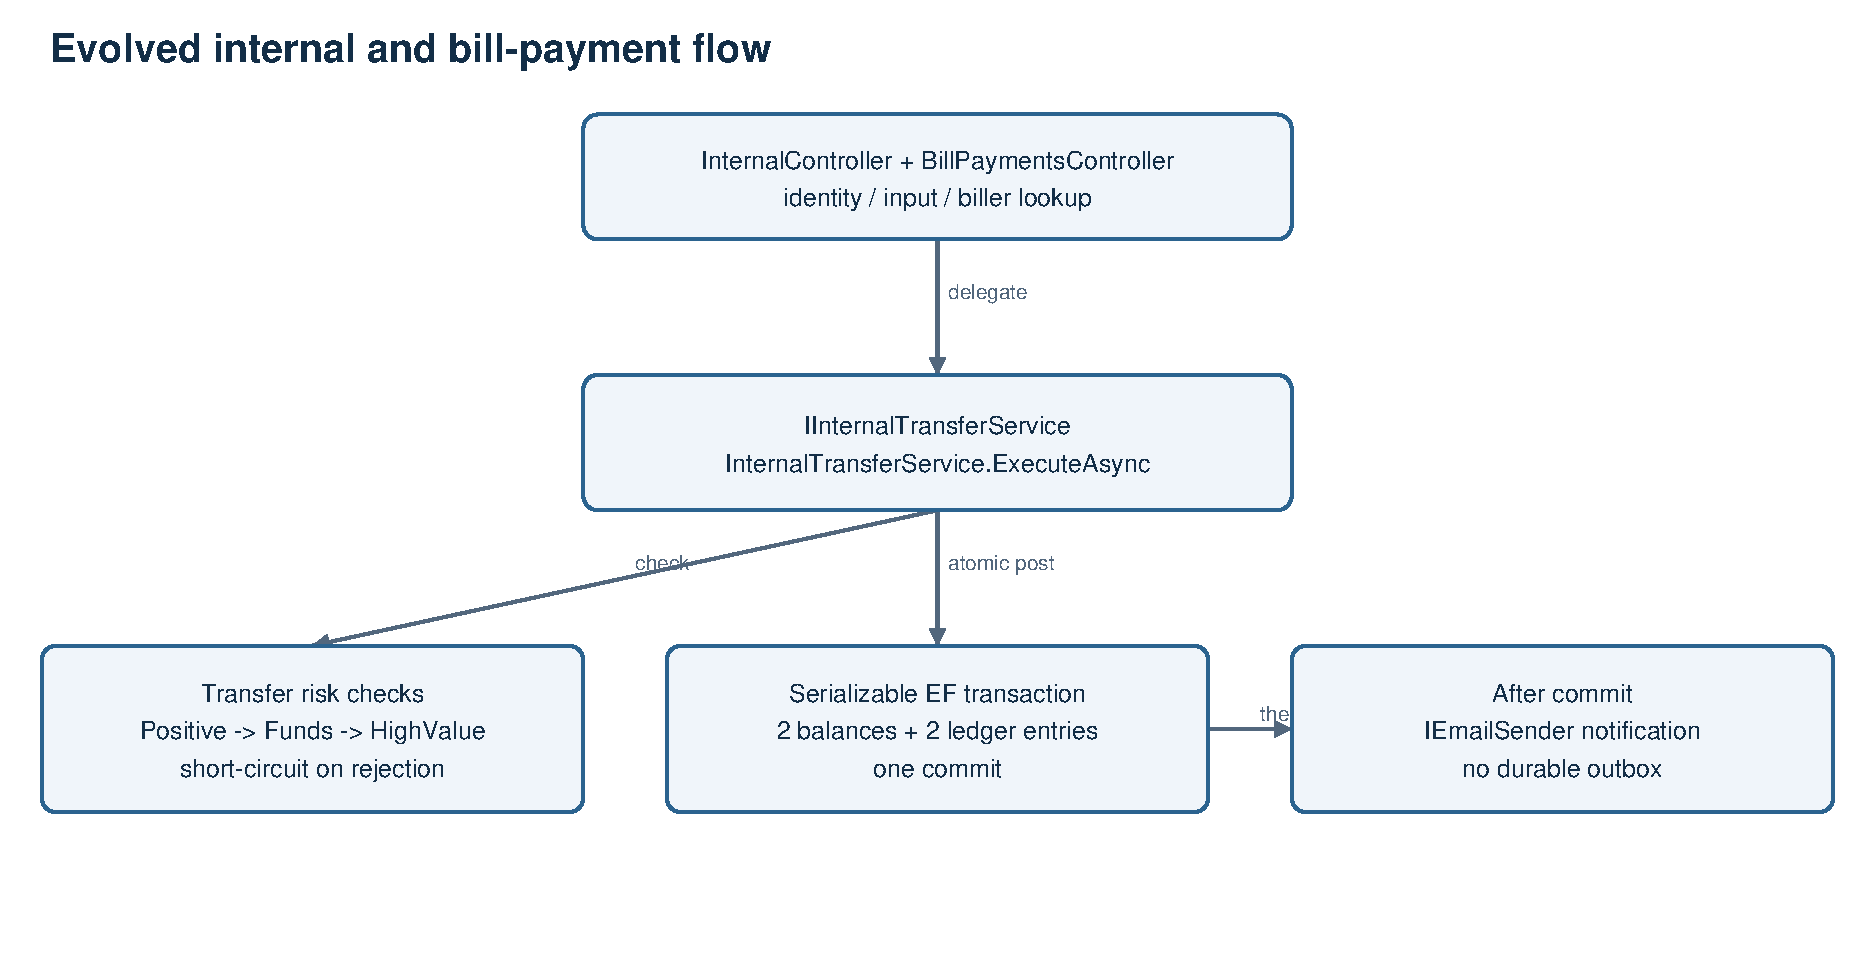
\includegraphics[width=.94\linewidth]{Part2/diagrams/evolved.pdf}\par{\small Figure 6. Final internal and bill-payment flow; CH03 adds the risk-chain branch.}\end{center}
\entry{Acceptance evidence}{Transfer/BillPayment ledger type, paired references, balanced amounts, account balances, ownership, missing/self destination, invalid precision/type/description, notification failure and SQL-trigger-induced rollback are tested with SQLite.}
\entry{Trade-off}{The service has no request-idempotency registry or durable notification outbox. SQL Server contention/deadlocks and operational recovery are not load-tested. Existing external/card/global paths retain their original behavior.}
\clearpage
\subsection{CH03: additional fraud-detection rule}
\entry{Requirement}{Reject internal or bill payments above the configurable inclusive single-transfer limit. A payment equal to the limit is allowed. Zero/negative limits are invalid configuration.}
\entry{Implementation}{Startup injects PositiveAmountRule, SufficientFundsRule and HighValueRule through ITransferRule. TransferRule checks its own condition and only forwards a successful request to its successor. ExecuteAsync evaluates the chain before balance changes.}
\entry{Pattern effect}{New Chain of Responsibility instance: Transfer risk checks. Atomic internal payment is extended by policy injection; its name and identity remain unchanged.}
\entry{Refactoring}{Extract linked handlers from policy checks. Additional risk conditions can be composed without enlarging controller branches. Request shape and account ownership remain service responsibilities.}
\entry{Before/after}{after\_change2 to after\_change3. Exact patch and final manifest: \path{Part2/changes/Change3/}; source: \path{Part2/code/}.}
\begin{center}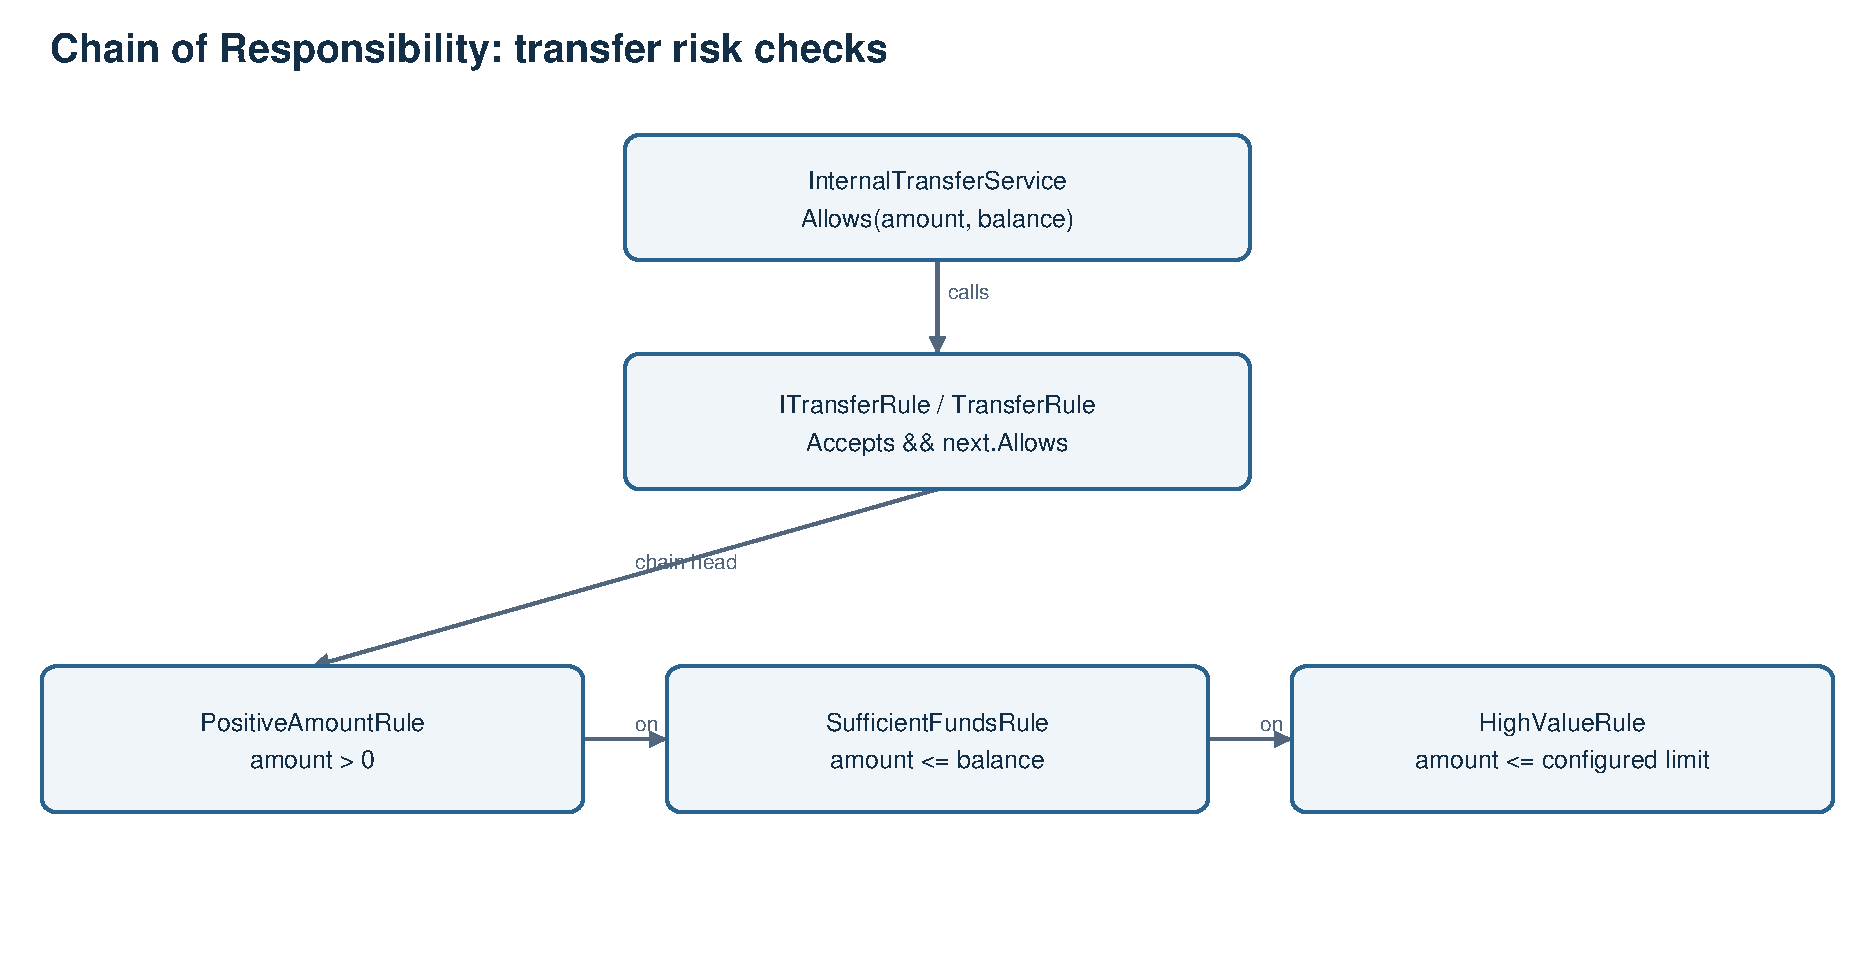
\includegraphics[width=.94\linewidth]{Part2/diagrams/chain.pdf}\par{\small Figure 7. Explicit handler succession with short-circuit rejection.}\end{center}
\entry{Acceptance evidence}{Limit boundary and breach, insufficient funds, invalid/zero/negative amounts, invalid policy configuration and short-circuit behavior are tested. This is a deterministic risk rule, not an AML model or a global payment-fraud engine.}
\clearpage
\subsection{Updated counts and comparable metrics}
\begin{tabularx}{\linewidth}{@{}Lp{15mm}p{19mm}p{20mm}p{19mm}@{}}\toprule
Snapshot & Types & Instances & Concrete & Symbols\\\midrule
original & 3 & 6 & 6 & 22\\
after\_change1 & 4 & 7 & 8 & 27\\
after\_change2 & 4 & 8 & 9 & 31\\
after\_change3 & 5 & 9 & 12 & 36\\
\bottomrule\end{tabularx}
The three rejected candidates and one uncertain framework interpretation remain separate observations in every snapshot. Removed instances are not invented: the legacy posting service continues to serve other flows, while the new atomic service has a separate collaboration name.

\begin{tabularx}{\linewidth}{@{}Lp{17mm}p{30mm}p{37mm}@{}}\toprule
Snapshot & Files & Source LOC & Max function CC\\\midrule
original & 4 & 363 & 9\\
after\_change1 & 6 & 444 & 9\\
after\_change2 & 10 & 558 & 17\\
after\_change3 & 11 & 601 & 17\\
\bottomrule\end{tabularx}
\entry{Measurement method}{Lizard 1.21.0; fixed union of changed production C\# paths in \code{data/metrics_scope.json}. Missing/new files contribute zero before introduction. Excludes tests, migrations and Razor markup. Source LOC excludes blank/comment lines according to Lizard. Maximum function CC is the maximum reported function value.}
\entry{Interpretation}{LOC increases because the changes add behavior, validation and extensibility. The maximum CC rises from 9 to 17 when the atomic service centralizes validation and transaction control; it does not drop after CH03 because request-validation branches remain. The result is reported honestly rather than treating pattern use as automatic complexity reduction.}
\begin{tabularx}{\linewidth}{@{}p{51mm}p{31mm}L@{}}\toprule
Verification scope & Actual result & Evidence\\\midrule
Original source suite & 129/129 passed & data/test\_result/baseline.txt\\
Same suite / final assemblies & 129/129 passed & data/test\_result/regression.txt\\
New feature cases & 26/26 passed & data/test\_result/evolution.txt\\
Full web + SQL Server + providers & Not run & Local configuration required\\
Intermediate full test suites & Not separately run & Snapshots and final cumulative acceptance retained\\
\bottomrule\end{tabularx}
The hosted VSTest launcher could not inspect process metadata. The included reflection runner executes the actual Fact and InlineData cases, creates a fresh instance per case, awaits asynchronous methods and fails on unsupported/skipped cases. The original compiled test assembly was also executed against the changed production assemblies for regression. This is documented as a fallback runner, not mislabelled as a successful VSTest session.
\clearpage
\section{Part 3: Cross-language comparison}
\entry{Selected instances}{One representative for each confirmed pattern type: Notification transport (Adapter), Security header policy (Builder), Transfer posting (Service Layer), Second-factor login (Strategy), Transfer risk checks (Chain of Responsibility).}
\entry{Implementation scope}{Twenty production snippets and twenty separate test runners in Java, Python, JavaScript and C++. Identical TSV inputs/outputs are read from five shared fixture files. These reduced collaborations do not implement the entire banking web application.}
\begin{tabularx}{\linewidth}{@{}p{42mm}L@{}}\toprule
Pattern & Common specification and cases\\\midrule
Adapter & 3: accepted vendor status, failed status, vendor exception; verify application-to-vendor payload mapping.\\
Builder & 4: add/overwrite, remove existing header, reject empty key, remove absent header.\\
Service Layer & 5: positive, negative and zero signed posting, absent account and baseline overdraft behavior; check notification count.\\
Strategy & 4: valid/invalid authenticator; valid one-time and invalid recovery code. Providers are injected test doubles.\\
Chain of Responsibility & 7: normal, exact limit, above limit, insufficient funds, zero/negative amount, invalid limit.\\
\bottomrule\end{tabularx}
\entry{Behavioral reductions}{Integer minor units avoid cross-language floating-point differences. The posting snippet intentionally preserves the old signed-posting behavior; it is not the new safe internal-payment service. The Builder snippet returns a copy, whereas the original returns its policy object. Portable Identity providers are test doubles; native C\# tests separately verify actual Identity recovery-code consumption.}
\entry{Measurement protocol}{Compile first; one warm-up; five measured fresh processes on the same host. Median includes startup, fixture reading and assertions; compilation excluded. Production files exclude all test doubles and runners. Lizard 1.21.0 records NLOC and maximum function CC.}
\entry{Result}{All 20 implementations pass: 92/92 shared cases. Raw samples: \path{Part3/evidence/raw_timings.json}. Commands, versions and results: \path{data/cross_language.csv}.}
\clearpage
\subsection{Measured results}
{\small
\begin{tabularx}{\linewidth}{@{}Lp{22mm}p{10mm}p{9mm}p{14mm}p{22mm}@{}}\toprule
Pattern & Language & LOC & CC & Tests & Median ms\\\midrule
Adapter & Java & 12 & 3 & 3/3 & 41.1992\\
Adapter & Python & 9 & 3 & 3/3 & 18.6954\\
Adapter & JavaScript & 8 & 3 & 3/3 & 52.787\\
Adapter & C++ & 13 & 3 & 3/3 & 1.9651\\
Builder & Java & 14 & 2 & 4/4 & 39.5423\\
Builder & Python & 13 & 2 & 4/4 & 18.0265\\
Builder & JavaScript & 11 & 2 & 4/4 & 50.5045\\
Builder & C++ & 14 & 2 & 4/4 & 1.3886\\
Service Layer & Java & 17 & 2 & 5/5 & 48.8393\\
Service Layer & Python & 12 & 2 & 5/5 & 18.9166\\
Service Layer & JavaScript & 12 & 2 & 5/5 & 56.1989\\
Service Layer & C++ & 21 & 2 & 5/5 & 1.9026\\
Strategy & Java & 19 & 1 & 4/4 & 51.0588\\
Strategy & Python & 18 & 1 & 4/4 & 19.3895\\
Strategy & JavaScript & 13 & 1 & 4/4 & 51.1246\\
Strategy & C++ & 21 & 1 & 4/4 & 1.431\\
Chain & Java & 27 & 3 & 7/7 & 39.2916\\
Chain & Python & 19 & 3 & 7/7 & 19.5286\\
Chain & JavaScript & 17 & 3 & 7/7 & 54.2148\\
Chain & C++ & 27 & 3 & 7/7 & 1.5844\\
\bottomrule\end{tabularx}
}
These measurements describe small process-level demonstrations on the recorded host. Runtime initialization can dominate the useful work. They do not establish a steady-state throughput result, production latency, or a universal fastest language.

\entry{Reproduction}{Each language folder supplies its exact compile/run command. \code{tools/measure.py} rebuilds the comparison CSV and raw timing evidence. Tests are deliberately separate from production source, as required by the faculty schema.}
\clearpage
\subsection{Language and technology discussion}
\begin{tabularx}{\linewidth}{@{}p{29mm}L@{}}\toprule
Language & Observed implementation characteristics\\\midrule
Java & Explicit interfaces and abstract classes express the Strategy and Chain contracts. Garbage collection removes manual ownership management; JDK compilation is excluded from measured process times.\\
Python & Duck typing, injected callables and small classes express the same collaborations with less declaration syntax. Runtime type flexibility does not remove the need for the same edge-case tests.\\
JavaScript & Objects, methods, callbacks and Map implement contracts structurally. Explicit test failures enforce behavior because compile-time interface checking is absent in plain JavaScript.\\
C++ & Virtual interfaces express substitutability; unique\_ptr owns the risk chain. References and callbacks connect collaborators without a managed runtime. Integer sizes and object lifetime remain explicit concerns.\\
\bottomrule\end{tabularx}
The design intent remains stable across languages: translate a boundary (Adapter), incrementally assemble a policy (Builder), coordinate an application operation (Service Layer), substitute a verification behavior (Strategy), or pass a request through successive checks (Chain of Responsibility). Language syntax and memory/runtime models change the expression, not the reason for the collaboration.

A Service Layer provides an application-operation boundary and coordinates the response to each use case, matching Fowler/Stafford's catalogue description. EF transactions provide atomicity on a supported relational provider; that is why the rollback test uses SQLite rather than relying on the non-relational EF InMemory provider. Identity exposes a recovery-code sign-in API, so the extension delegates to the framework instead of implementing its own code-consumption logic. References are listed at the end and in \code{REFERENCES.md}.
\clearpage
\section{LLM records and human verification}
\entry{Current-session use}{The assistant inspected source, proposed the changes, generated code/diagrams/documentation and ran automated checks. The user request and follow-up instructions are saved under \code{data/llm/}.}
\entry{Model/access tier}{The exact displayed model identity and free/public access tier were not independently verified. No free-tier or historic Gemini experiment is claimed. The work date is 2026-10-24.}
\entry{Inputs and outputs}{Each part has an input manifest, a newly authored analysis artifact and a verification note. The canonical \code{llm.csv} references them. These are not presented as a byte-exact export of the entire conversation.}
\begin{tabularx}{\linewidth}{@{}p{66mm}L@{}}\toprule
Claim / draft risk & Evaluation and correction\\\midrule
Email notification implies Observer & Incorrect; source directly invokes IEmailSender. Record Adapter, not Observer.\\
Entity Framework means custom Repository & Incorrect in the stated scope; DbContext is a dependency abstraction, not a student-written repository class.\\
Authenticator 2FA is the new mechanism & Incorrect; it already exists upstream. CH01 adds recovery-code authentication as an alternative second factor.\\
Two successful single postings are atomic & Incorrect under partial failure. CH02 replaces the original internal flow with one relational transaction.\\
Patterns necessarily lower complexity & Unsupported; measured max CC rises from 9 to 17, and LOC grows. Report the actual values.\\
Tests prove live bank deployment & Incorrect; tests use synthetic accounts and local providers. Browser/SQL Server/external integrations are not end-to-end verified.\\
\bottomrule\end{tabularx}
\entry{Evidence}{Qualified source mappings and patch manifests support structural claims. Native and portable test logs support the stated behavior. Automated checks do not establish individual student authorship, faculty approval or human review.}
\entry{Required final provenance action}{Export the actual conversation with its exact prompt, supplied context and raw responses, or conduct a real documented free/public-tool session if required by the faculty. Add the real human reviewer and evaluation. Do not reconstruct missing history or assign an invented model/date/reviewer.}
\clearpage
\section{Findings, contributions and references}
\subsection{Evidence-supported findings}
\begin{enumerate}
\item The pinned baseline contains Adapter, Builder and four named architectural service collaborations in the inspected scope. Framework use is not automatically a new GoF instance.
\item Recovery authentication extends an existing Identity flow through Strategy. Identity owns recovery-code generation and redemption.
\item Bill payments reuse a real refactoring of the internal transfer path. A forced SQL failure leaves both balances and ledger entries unchanged in the relational test.
\item Risk handling becomes a configurable linked collaboration. Its scope is the new internal/bill service, not all bank operations.
\item All original regression cases and all added feature/portable cases pass under the documented execution procedures. Metrics and provenance gaps remain explicitly visible.
\end{enumerate}
\subsection{Limitations and contributions}
The package does not establish a live SQL Server/browser/provider deployment, performance under concurrency, replay-safe bill payments, invoice deduplication, durable notifications or a global fraud engine. The legacy framework and dependencies need a separate modernization effort before any real deployment.

The banking-team identities, actual work allocation, faculty approval and human verification were not supplied. \code{team.json} remains empty rather than borrowing a roster from another project. The source generation, analysis and automated execution in this package were assistant-assisted; students should review the code and record their actual contributions.
\subsection{References}
\begin{enumerate}
\item BankSystem, MIT licensed source, pinned commit. \url{https://github.com/banksystembg/BankSystem}
\item Gamma, Helm, Johnson and Vlissides. \emph{Design Patterns: Elements of Reusable Object-Oriented Software}. Addison-Wesley, 1994.
\item Fowler/Stafford, Service Layer. \url{https://martinfowler.com/eaaCatalog/serviceLayer.html}
\item Microsoft, EF Core transactions. \url{https://learn.microsoft.com/en-us/ef/core/saving/transactions}
\item Microsoft, SignInManager recovery-code API. See exact URL in \code{REFERENCES.md}.
\item Lizard 1.21.0, source-code metrics. \url{https://github.com/terryyin/lizard}
\item User-supplied 23CSE455 case-study instructions and LaTeX template, read 2026-10-24.
\end{enumerate}
\clearpage
\section{Team folder and datasets}
The latest faculty instruction asks for one consolidated report and one authoritative dataset directory. The part folders organize source, changes, diagrams and evidence; they are not separate submissions. The folder name below must be replaced with the exact team code before upload.
\begin{lstlisting}
BankingCaseStudy/
  README.md
  UPLOAD_TO_GITHUB.md
  BankingCaseStudy_Report.tex
  BankingCaseStudy_Report.pdf
  team.json
  data/
    code/                       original source
    patterns.csv
    pattern_counts.csv
    patterns_evolution.csv
    participant_counts.csv
    evolution_metrics.csv
    cross_language.csv
    llm.csv
    test_result/                executed C# logs
  Part1/
    evidence/                   module and role audit
    pattern_architecture/       drawio + SVG + PDF
    llm/
  Part2/
    code/                       evolved source
    changes/Change1..Change3/    patches + hashes
    tests/                      feature cases
    diagrams/                   drawio + SVG + PDF
    llm/
  Part3/
    adapter/ builder/ service_layer/
    strategy/ chain_of_responsibility/
      java/ python/ javascript/ cpp/
    test-cases/                 shared TSV fixtures
    evidence/                   raw times + outcomes
    llm/
  tools/                        verification + measurement
\end{lstlisting}
\textbf{GitHub screenshot status}\par
No GitHub upload was performed because the user requested files to upload personally. A genuine repository screenshot cannot be supplied before that upload. After uploading, capture the team folder, add the image here and recompile the PDF. The local hierarchy above is not labelled as a GitHub screenshot.
\end{document}
